\documentclass{article}
\usepackage[UTF8]{ctex}
\usepackage{fontspec}
\setmainfont{Times New Roman}
\setsansfont{Arial}
\setmonofont{Courier New}
\usepackage[english]{babel}
\usepackage{graphicx}
\usepackage{float}
\usepackage{hyperref}
\usepackage{amsmath}
\usepackage{amssymb}
\usepackage{booktabs}
\usepackage{multirow}
\usepackage{array}
\usepackage{geometry}
\geometry{a4paper, margin=1in}
\usepackage{unicode-math}
\setmonofont{DejaVu Sans Mono}
\usepackage{pdfpages}
\usepackage{listings}
\lstset{
    basicstyle=\ttfamily\small,
    breaklines=true,
    postbreak=\raisebox{0ex}[0ex][0ex]{\ensuremath{\hookrightarrow\space}},
    columns=fullflexible,
    frame=single,
    showstringspaces=true,
    keepspaces=true,
    tabsize=4,
    xleftmargin=2em,
    xrightmargin=2em
}

\usepackage{fancyvrb}
\usepackage{fancyhdr}
\usepackage{lastpage}
\pagestyle{fancy}
\fancyhf{}
\fancyhead[C]{Xiamen University Malaysia}
\fancyfoot[C]{\thepage/\pageref{LastPage}}
% \fancyfoot[C]{\thepage/30}
\fancyhead[R]{\leftmark}
\fancyhead[L]{G0191 Face Recognition}


\title{PCA in Face Recognition Project Report}
\date{2025 February Semester Week 5}
\author{
    Liu Zhen (AIT2409033) \\
    Cui Zeyu (DSC2409006) \\ \\
    \href{https://github.com/zeyu10/FaceRecognition}{Project Website (GitHub)}
}

\begin{document}
\maketitle

\tableofcontents
\newpage

\section{Introduction}
In today's digital era, face recognition technology, as one of the core technologies in the field of biometrics, has been widely applied in various domains due to its uniqueness, convenience, and efficiency. From real-time identity recognition in security surveillance to intelligent management of access control systems, and even to face payment in the financial sector, face recognition technology is profoundly changing the way people live and work.

This project focuses on designing and implementing a face recognition system based on Principal Component Analysis (PCA). The goal is to provide a reliable and efficient solution for identity recognition in various scenarios. By collecting and processing a large amount of face data, using PCA to extract key features, and combining advanced classification algorithms, the system can accurately identify individuals, providing strong support for practical applications.
\newpage
\section{Usage Instructions}

\subsection{Environment Setup and Data Preparation}

\subsubsection{Installing Dependencies}
The system is developed based on Python, so ensure that the Python environment is installed before running the project. The project mainly depends on libraries such as \texttt{OpenCV}, \texttt{NumPy}, and \texttt{PyQt5}. You can use the \texttt{pip} tool to install these dependencies by executing the following commands in the command line: \texttt{pip install opencv-python}, \texttt{pip install numpy}, and \texttt{pip install PyQt5}.

\subsubsection{Collecting Face Data}
According to the project requirements, at least 100 face images from more than 20 individuals need to be collected. The collected face images should be categorized by individual and stored in separate folders. The folder names serve as identifiers for the corresponding individuals, and the image formats supported are \texttt{.jpg}, \texttt{.jpeg}, and \texttt{.png}. Ensure that the image quality is good and the background is relatively simple to improve the accuracy of subsequent recognition.

\subsection{Project Overview}

\subsubsection{Project Structure Overview}
\begin{lstlisting}[basicstyle=\scriptsize\ttfamily]
FaceRecognition/
│
├── Config.py           # Configuration file containing system parameters and constants
├── Dataset.py          # Dataset processing module, responsible for data import, processing, and saving
├── FaceDetector.py     # Face detection module, responsible for detecting and preprocessing face images
├── Recognizer.py       # Recognition module, implementing PCA and kNN algorithms
├── MainWindow.py       # Main interface module, providing user interface and system function integration
│
├── Caffemodel/              # Pre-trained deep learning model files
│   ├── deploy.prototxt      # Model configuration file
│   └── res10_300x300_ssd_iter_140000.caffemodel
│                            # Model weight file
│
├── Dataset/                 # Dataset folder, storing original images and preprocessed data
│   ├── Att_Faces/           # Contains original images from the Att_Faces dataset
│   ├── Dataset_Personal/    # Contains personal dataset with background
│   ├── Dataset_Pure/        # Contains pure personal dataset
│   ├── Dataset_Personal_Big.pkl    # Preprocessed file for the large personal dataset
│   ├── Dataset_Personal_Small.pkl  # Preprocessed file for the small personal dataset
│   └── Dataset_Personal_with_AttFaces.pkl
│                                   # Preprocessed file for the personal dataset including Att_Faces
│
├── Report.pdf               # Project report document
\end{lstlisting}

\subsubsection{File Function Descriptions}

\paragraph{1. Config.py}
\begin{itemize}
    \item \textbf{Function}: Configuration file defining constant parameters used in the system.
    \item \textbf{Key Parameters}:
    \begin{itemize}
        \item \texttt{FACE\_EXTEND\_FACTOR}: Face region extension factor.
        \item \texttt{TRAIN\_RATIO}: Ratio for splitting the dataset into training and testing sets.
        \item \texttt{KEEP\_COMPONENTS}: Proportion of principal components retained in PCA.
        \item \texttt{RECOGNITION\_SIZE}: Uniform size for face images.
        \item \texttt{CANDIDATE\_K}: List of candidate k values for the kNN algorithm.
    \end{itemize}
\end{itemize}

\paragraph{2. Dataset.py}
\begin{itemize}
    \item \textbf{Function}: Dataset processing module, responsible for data import, processing, and saving.
    \item \textbf{Core Functions}:
    \begin{itemize}
        \item \texttt{import\_dataset}: Imports face image data from folders and preprocesses it.
        \item \texttt{save\_dataset}: Saves the dataset as a \texttt{.pkl} file.
        \item \texttt{load\_dataset}: Loads the dataset from a \texttt{.pkl} file.
        \item \texttt{split\_dataset}: Splits the dataset into training and testing sets.
    \end{itemize}
\end{itemize}

\paragraph{3. FaceDetector.py}
\begin{itemize}
    \item \textbf{Function}: Face detection module, responsible for detecting and preprocessing face images.
    \item \textbf{Core Functions}:
    \begin{itemize}
        \item \texttt{detect\_faces}: Uses a deep learning model to detect faces.
        \item \texttt{get\_most\_confident\_face\_region}: Retrieves the most confident face region.
        \item \texttt{enhance\_image}: Enhances the image and removes the background.
    \end{itemize}
\end{itemize}

\paragraph{4. Recognizer.py}
\begin{itemize}
    \item \textbf{Function}: Recognition module, implementing PCA and kNN algorithms.
    \item \textbf{Core Functions}:
    \begin{itemize}
        \item \texttt{fit}: Uses PCA for feature extraction.
        \item \texttt{evaluate}: Evaluates the model's accuracy.
        \item \texttt{predict}: Uses the kNN algorithm for face recognition.
        \item \texttt{kNNR\_classifier}: Implementation of the kNN classifier.
    \end{itemize}
\end{itemize}

\paragraph{5. MainWindow.py}
\begin{itemize}
    \item \textbf{Function}: Main interface module, providing user interface and system function integration.
    \item \textbf{Core Functions}:
    \begin{itemize}
        \item \texttt{MainWindow}: Main window class, integrating data import, model training, camera operations, and other functions.
        \item \texttt{CameraWindows}: Camera window class, providing real-time face detection and recognition functions.
        \item \texttt{slot\_add\_face}: Adds face data to the interface.
        \item \texttt{on\_train\_model}: Trains the model and displays training progress.
    \end{itemize}
\end{itemize}

\paragraph{6. Caffemodel/}
\begin{itemize}
    \item \textbf{Function}: Stores pre-trained deep learning model files.
    \item \textbf{Files}:
    \begin{itemize}
        \item \texttt{deploy.prototxt}: Model configuration file.
        \item \texttt{res10\_300x300\_ssd\_iter\_140000.caffemodel}: Model weight file.
    \end{itemize}
\end{itemize}

\paragraph{7. Dataset/}
\begin{itemize}
    \item \textbf{Function}: Stores original images of the dataset and preprocessed dataset files.
    \item \textbf{Contents}:
    \begin{itemize}
        \item \texttt{Att\_Faces/}: Stores original images from the Att\_Faces dataset, totaling \textbf{400} images.
        \item \texttt{Dataset\_Personal\_With\_Background/}: Stores the group members' dataset with background, totaling \textbf{65} images.
        \item \texttt{Dataset\_Pure/}: Stores the pure personal dataset, totaling \textbf{103} images.
        \item \texttt{Dataset\_Personal\_Big.pkl}: Stores the preprocessed file for the large personal dataset
        \begin{itemize}
            \item Includes \texttt{Dataset\_Personal\_With\_Background/} + \texttt{Dataset\_Pure/} datasets.
        \end{itemize}
            \item \texttt{Dataset\_Personal\_Small.pkl}: Stores the preprocessed file for the small personal dataset
        \begin{itemize}
            \item Only includes the \texttt{Dataset\_Personal\_With\_Background/} dataset.
        \end{itemize}
        \item \texttt{Dataset\_Personal\_with\_Attfaces.pkl}: Stores the preprocessed file for the complete personal dataset
        \begin{itemize}
            \item Includes \texttt{Dataset\_Personal\_With\_Background/} + \texttt{Dataset\_Pure/} + \texttt{Att\_Faces/} datasets.
        \end{itemize}
    \end{itemize}
\end{itemize}

\subsection{Project Operation Process}

\subsubsection{Starting the Project}
Locate the \texttt{MainWindow.py} file in the project directory and run the command \texttt{python MainWindow.py} in the command line to start the face recognition system. After the system starts, the main window will pop up, integrating functions such as data import, model training, camera operations, dataset management, and displaying the image area and data table.

\begin{figure}[H]
    \centering
    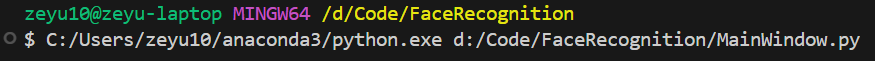
\includegraphics[width=0.8\textwidth]{Img/PixPin_2025-03-09_00-37-52.png}
    \caption{Command line starting the main window of the project}
\end{figure}

\subsubsection{Importing Data}
\begin{itemize}
    \item Click the \texttt{Import From Folder} button in the main window, and the system will pop up a file selection dialog. Navigate to the folder storing face images in the dialog, select the folder, and click "OK".
    \item At this point, the system will pop up a query box asking whether to remove the face background. If "Yes" is selected, the system will use image processing techniques to remove the face background in subsequent processing; if "No" is selected, the original image background will be retained.
    \item The system starts reading image files from the selected folder and its subfolders. For images that are too large (pixels exceeding 62500), the system will perform face detection based on the \texttt{dnn} module of \texttt{OpenCV}, obtain the most confident face region, and extend and crop it according to the \texttt{FACE\_EXTEND\_FACTOR} parameter in the configuration file. Then, the image will be uniformly adjusted to the size of \texttt{RECOGNITION\_SIZE} (100x100).
    \item The processed image data will be stored in the system's dataset. At the same time, the data table in the main window will display the ID, name (determined by the folder name), path, and checkbox for whether to add to the model for each image.
\end{itemize}

\begin{figure}[H]
    \centering
    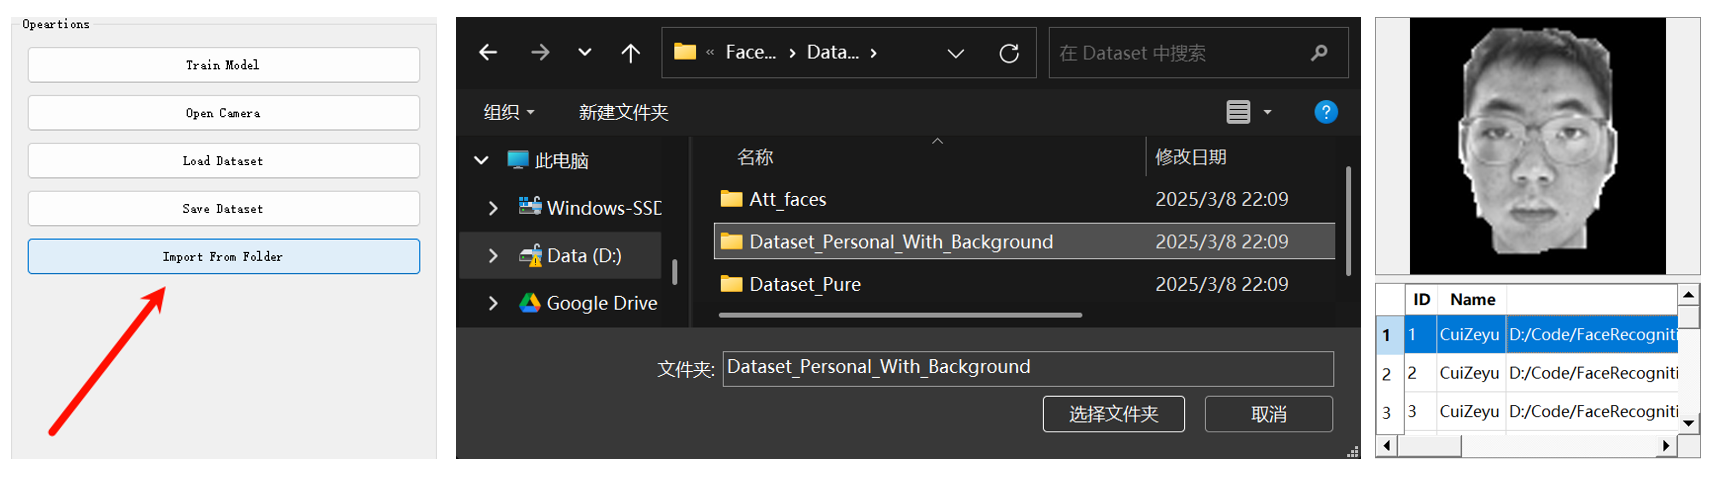
\includegraphics[width=0.8\textwidth]{Img/PixPin_2025-03-09_00-48-16.png}
    \caption{Data import interface}
\end{figure}

\subsubsection{Model Training}
\begin{itemize}
    \item Before training the model, ensure that enough face data has been imported into the data table. If the dataset is empty, clicking the \texttt{Train Model} button will pop up an error prompt box, reminding the user to import data first.
    \item After confirming the data is correct, click the \texttt{Train Model} button, and the system will start model training. During the training process, the progress bar at the bottom of the main window will display the progress in real time.
    \item Model training includes several key steps: first, processing the imported data to extract key features; then calculating related parameters such as the mean face, covariance matrix, eigenvalues, and eigenvectors; finally, evaluating the model to determine its performance metrics.
    \item After training is completed, the status bar of the main window will display the time spent on training and the accuracy of the model, allowing users to understand the training effect of the model.
    \item Multiple folders can be imported in the main window for training and recognition.
\end{itemize}

\begin{figure}[H]
    \centering
    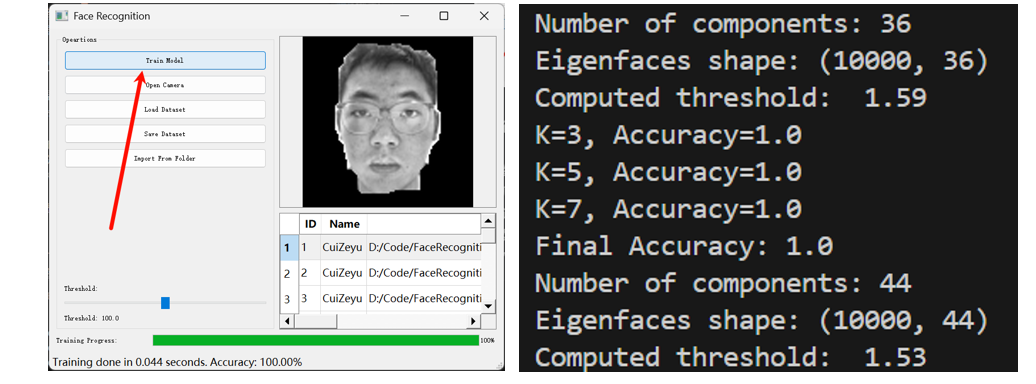
\includegraphics[width=0.8\textwidth]{Img/PixPin_2025-03-09_00-52-21.png}
    \caption{Model training interface}
\end{figure}

\subsubsection{Starting the Camera for Recognition}
\begin{itemize}
    \item Click the \texttt{Open Camera} button in the main window. If the camera is opened for the first time, the system will pop up a camera selection window, listing the available camera devices on the current device. Users can select the corresponding camera device according to the actual situation (if there is only one camera device, the system will automatically select and open it). After the camera window is opened, users can view the camera's live feed in real time.
    \item In the camera window, click the \texttt{Recognize Face} button. If the model has been successfully trained, the button will change to \texttt{Stop Recognizing}, and the face recognition function will be enabled. The system will detect faces in the camera's live feed, and once a face is detected, it will perform a series of processing and recognition operations on it.
    \item The recognition results will be displayed on the camera feed in real time. If a known individual is recognized, the individual's name will be displayed on the screen; if not recognized, \texttt{Stranger} will be displayed. In addition, in the small window on the right side of the camera window, the detected face image and the predicted matching image (if recognition is successful) will be displayed separately, allowing users to visually compare them.
    \item In the camera window, users can decide whether to remove the background of the detected face image by checking the \texttt{Remove Background} checkbox. After checking, the system will use relevant image processing algorithms to remove the background when processing face images, further improving recognition accuracy.
    \item Click the \texttt{Screenshot} button in the camera window to take a photo of the current camera feed. The photo will be saved in the program's running directory in the format \texttt{Screenshot\_yy\_dd\_hh\_mm\_ss.jpg}, and the status bar of the camera window will prompt the file name of the saved photo, making it easy for users to find.
\end{itemize}

\begin{figure}[H]
    \centering
    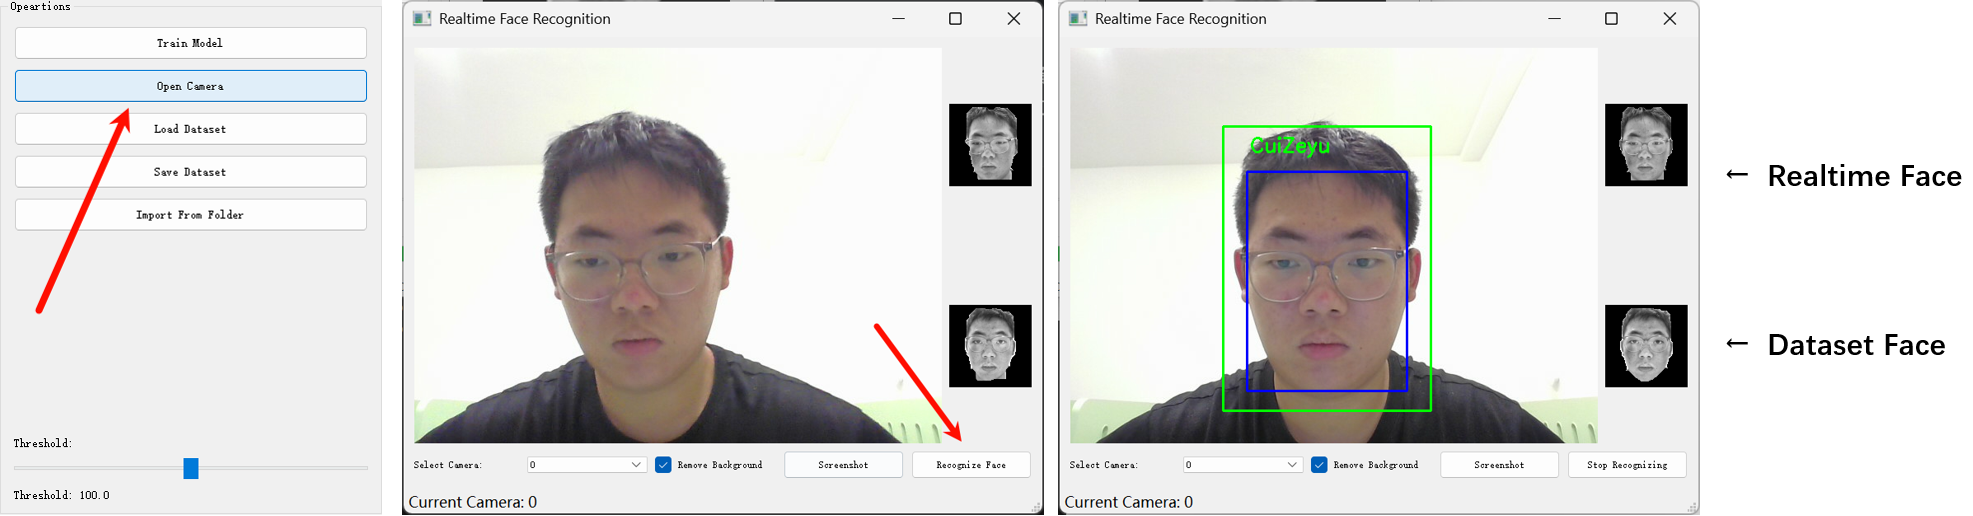
\includegraphics[width=0.8\textwidth]{Img/PixPin_2025-03-09_00-59-57.png}
    \caption{Camera test (Camera 0)}
\end{figure}

\begin{figure}[H]
    \centering
    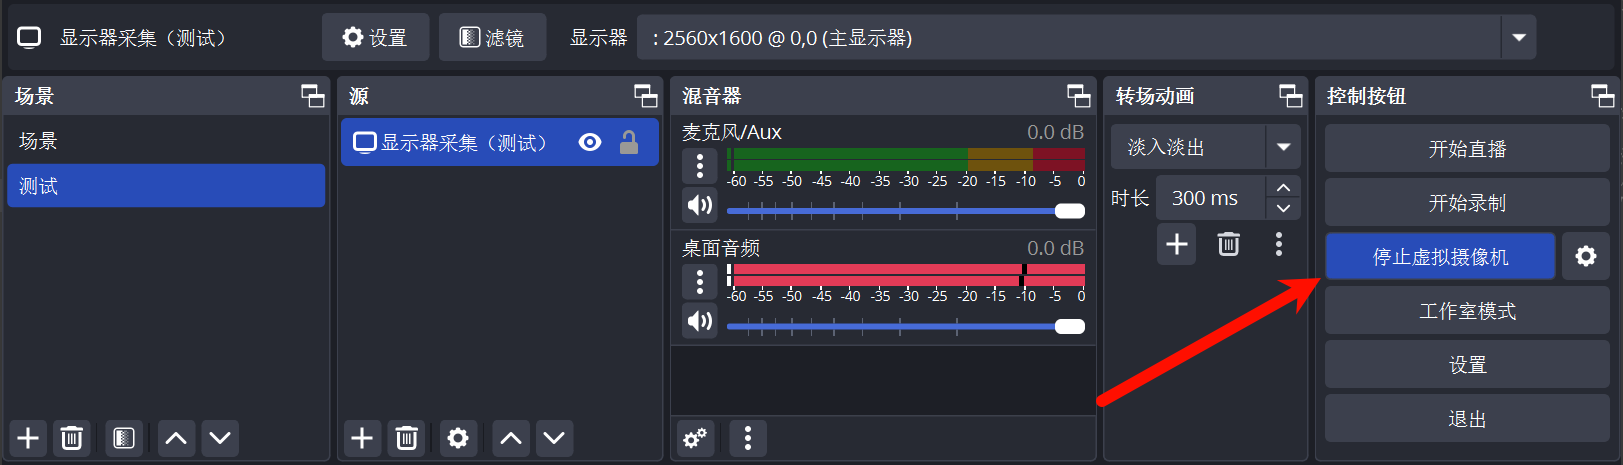
\includegraphics[width=0.8\textwidth]{Img/PixPin_2025-03-09_10-58-44.png}
    \caption{Local dataset test (Camera 1 or Camera 2, requires OBS virtual camera)}
\end{figure}

\begin{figure}[H]
    \centering
    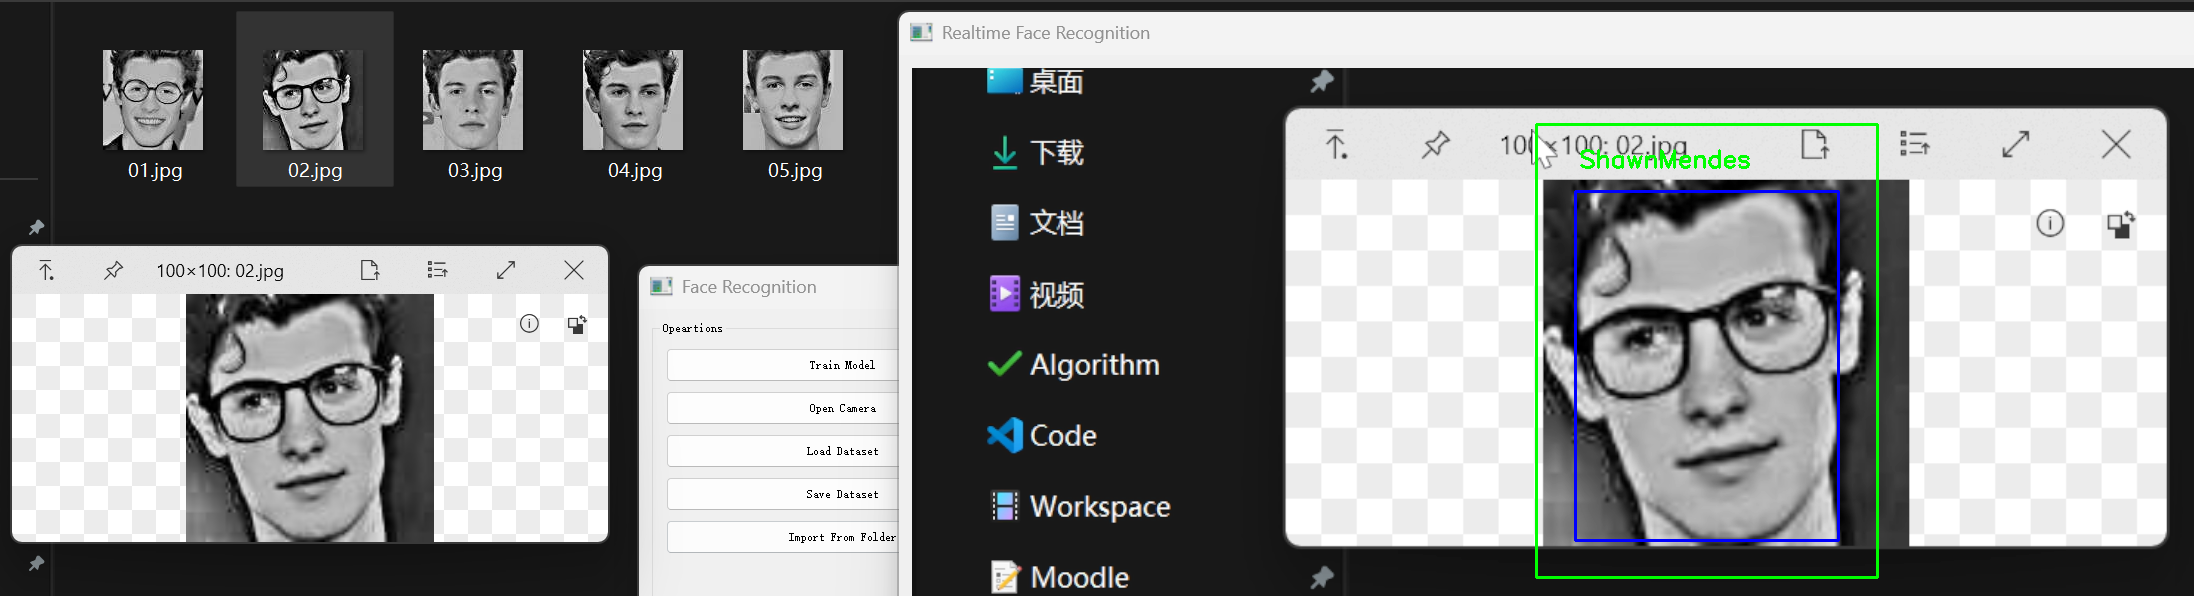
\includegraphics[width=0.8\textwidth]{Img/PixPin_2025-03-09_11-11-17.png}
    \caption{Local dataset test}
\end{figure}

\subsubsection{Adjusting Recognition Threshold}
\begin{itemize}
    \item In the left operation panel of the main window, users can see a slider control for adjusting the face recognition threshold. The threshold determines the system's requirement for similarity during the recognition process. The lower the threshold, the more relaxed the system's requirement for similarity, and the recognition results may include more misidentifications; the higher the threshold, the stricter the system's requirement for similarity, and the recognition results will be more accurate, but some correct recognitions with lower similarity may be missed.
    \item Users can adjust the threshold by dragging the slider. The slider's value ranges from 0 to 200, corresponding to a threshold range of 0.0 to 2.0. The system's default initial value is 100, corresponding to a threshold of 1.0. Users can adjust the threshold according to actual needs to achieve the best recognition effect.
    \item After adjusting the threshold, the system will update the recognition results in real time. Users can observe the recognition results in the camera window to determine whether the current threshold is appropriate.
\end{itemize}

\begin{figure}[H]
    \centering
    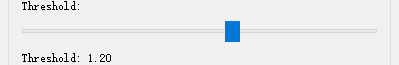
\includegraphics[width=0.6\textwidth]{Img/PixPin_2025-03-09_01-02-00.png}
    \caption{Adjusting recognition threshold interface}
\end{figure}

\subsubsection{Dataset Operations}
\begin{itemize}
    \item Click the \texttt{Save Dataset} button in the main window, and the system will pop up a file save dialog. Users can select the save path in the dialog and enter a file name (file format is \texttt{.pkl}). After clicking \texttt{Save}, the system will save the current dataset for later use.
\end{itemize}

\begin{figure}[H]
    \centering
    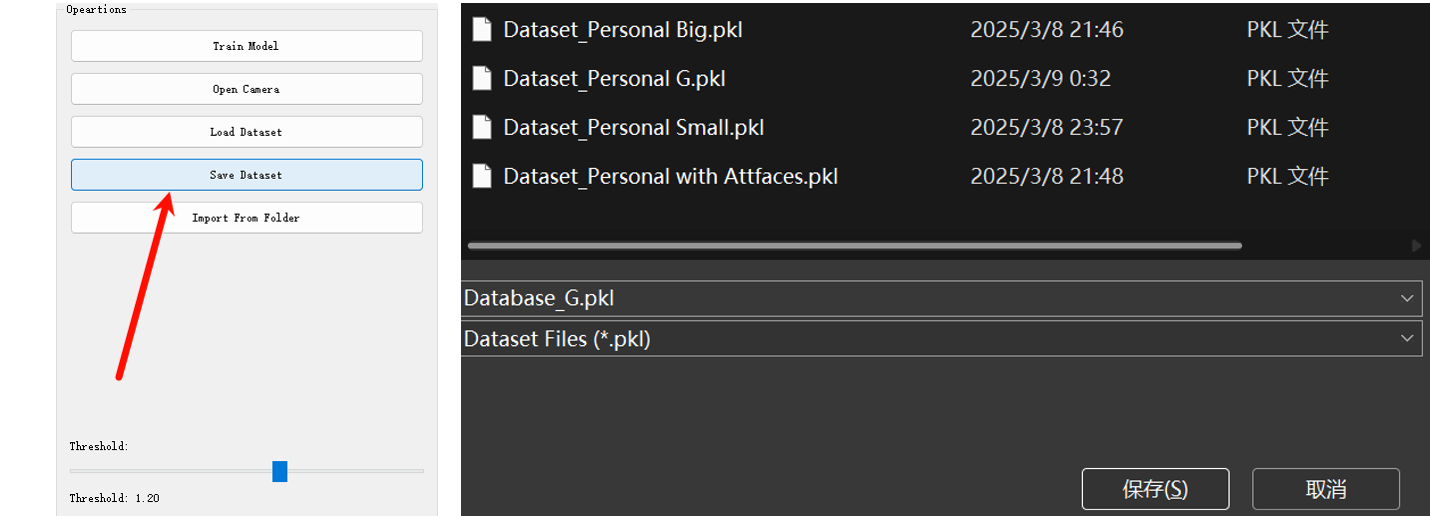
\includegraphics[width=0.8\textwidth]{Img/PixPin_2025-03-09_01-05-24.png}
    \caption{Saving dataset interface}
\end{figure}

\begin{itemize}
    \item Click the \texttt{Load Dataset} button, and the system will pop up a file selection dialog. Select the previously saved dataset file (\texttt{.pkl}), and the system will load the dataset, display the data in the data table of the main window, and update the relevant data index, allowing users to continue subsequent operations.
\end{itemize}

\begin{figure}[H]
    \centering
    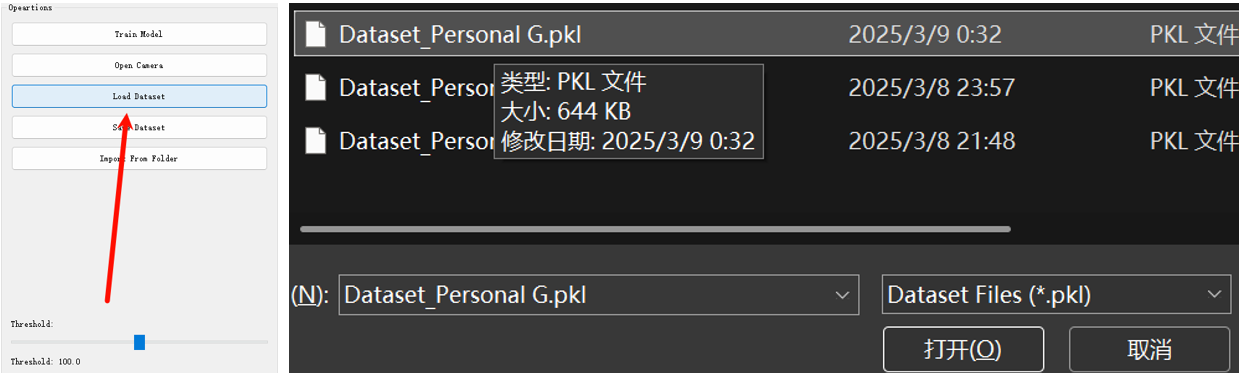
\includegraphics[width=0.8\textwidth]{Img/PixPin_2025-03-09_02-37-48.png}
    \caption{Loading dataset interface}
\end{figure}
\newpage
\section{Key Principles}

\subsection{Principal Component Analysis (PCA)}

\subsubsection{Basic Principles of PCA}
PCA is a powerful dimensionality reduction technique whose core goal is to project high-dimensional data onto a set of orthogonal principal components through linear transformation, so that the data can retain most of the variance information in a low-dimensional space. In the field of face recognition, each face image can be regarded as a high-dimensional vector, and these vectors constitute a high-dimensional data space. Through PCA, we can find the directions that can explain the data variance to the greatest extent, and the vectors corresponding to these directions are the so-called "eigenfaces". Using these eigenfaces, we can project high-dimensional face image data into a low-dimensional space, achieving dimensionality reduction while retaining key recognition features, thereby greatly reducing computational and storage requirements.

\subsubsection{Mathematical Principles of PCA}

\paragraph{Data Matrix Construction}
Assume there are \( m \) face images, each image is represented as an \( n \)-dimensional vector (assuming the image has been flattened into a one-dimensional vector), then a data matrix \( X \) of size \( n \times m \) can be constructed, where each column represents a face image vector.

\paragraph{Calculating the Mean Vector}
Calculate the mean vector \( \mu \) of the data matrix \( X \), the formula is:
\[
\mu = \frac{1}{m} \sum_{i=1}^{m} x_i
\]
where \( x_i \) represents the \( i \)-th image vector. The mean vector \( \mu \) represents the central tendency of the data. Geometrically, it is the centroid of all data points in the \( n \)-dimensional space. In face recognition, the mean face can be regarded as the average appearance of all faces, reflecting the basic features of the face.

\begin{figure}[H]
    \centering
    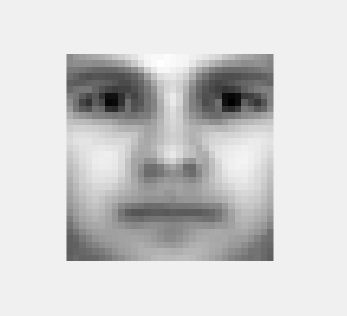
\includegraphics[width=0.5\textwidth]{Img/v2-918060b552a96c398d46f84574d5f2e4_1440w.png}
    \caption{"Mean face", the average of all faces}
\end{figure}

\paragraph{Data Centralization}
Subtract the mean vector \( \mu \) from each vector in the data matrix \( X \) to obtain the centered data matrix \( X_{\text{centered}} \), i.e.:
\[
X_{\text{centered}} = X - \mu \mathbf{1}^T
\]
where \( \mathbf{1} \) is a vector of size \( m \) with all elements being 1. The purpose of data centralization is to make the data distribution centered at the origin, eliminate the influence of data translation, and highlight the difference features of the data, preparing for subsequent feature extraction. After centralization, the mean of the data becomes zero, making the calculation of the covariance matrix more convenient and accurate.

\begin{figure}[H]
    \centering
    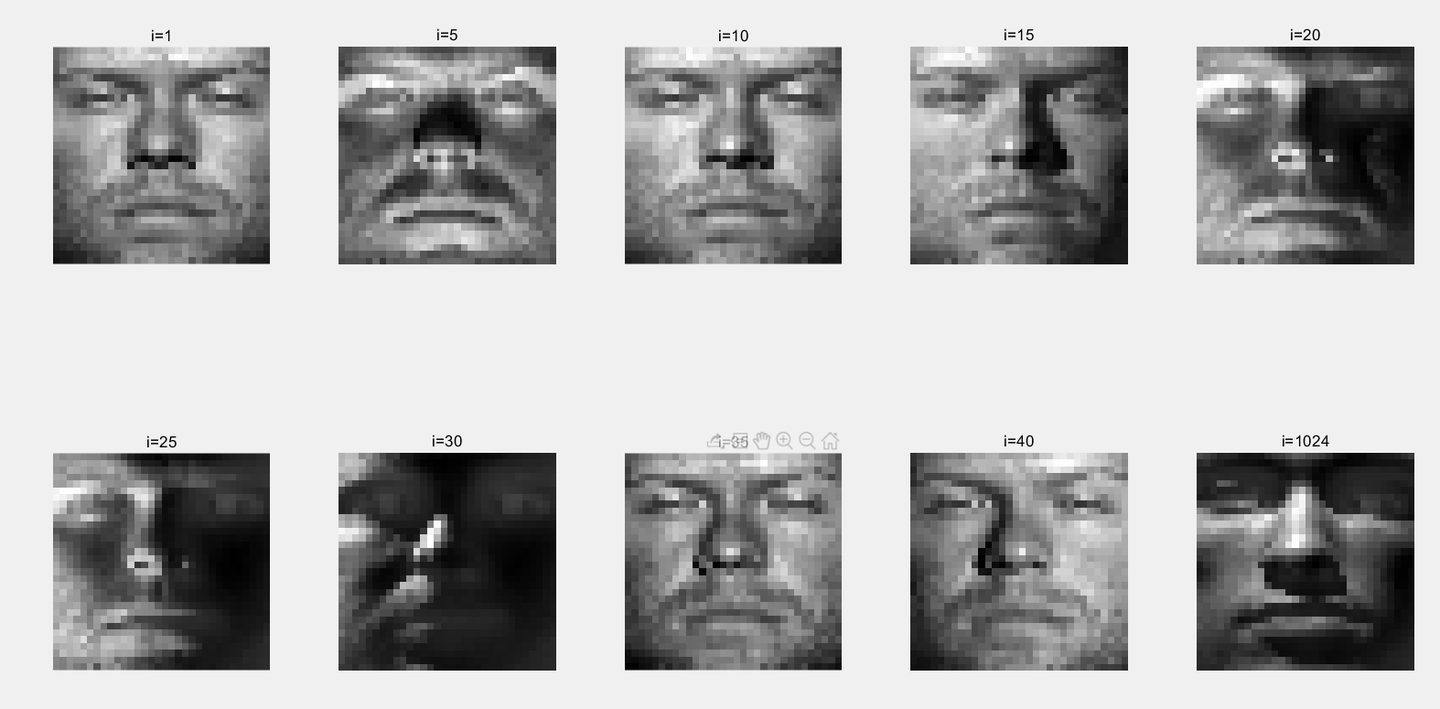
\includegraphics[width=0.8\textwidth]{Img/v2-65a459d10dbf796dcd4dbfec736c810a_1440w.png}
    \caption{Original data after subtracting the mean face to obtain the centered data}
\end{figure}

\paragraph{Calculating the Covariance Matrix}
Calculate the covariance matrix \( C \) of the centered data matrix \( X_{\text{centered}} \), the formula is:
\[
C = \frac{1}{m - 1} X_{\text{centered}} X_{\text{centered}}^T
\]
The covariance matrix \( C \) reflects the correlation between different dimensions of the data. The diagonal elements represent the variance of each dimension, and the off-diagonal elements represent the covariance between different dimensions. In face recognition, the covariance matrix describes the correlation between different pixels of the face image. For example, if two pixels have similar variation trends in different face images, the covariance between them will be large; otherwise, if the variation trends are independent, the covariance will be close to zero.

\paragraph{Solving Eigenvalues and Eigenvectors}
Perform eigenvalue decomposition on the covariance matrix \( C \) to solve its eigenvalues \( \lambda_i \) and eigenvectors \( v_i \), satisfying:
\[
C v_i = \lambda_i v_i
\]
The eigenvalue \( \lambda_i \) represents the variance of the data in the direction of the corresponding eigenvector \( v_i \), and the eigenvector \( v_i \) represents the direction of data variation in that direction. From the perspective of linear algebra, the eigenvectors are the invariant directions under the linear transformation defined by the covariance matrix \( C \), and the eigenvalues are the scaling factors in those directions. In face recognition, the eigenvectors (i.e., eigenfaces) represent the most variable directions in the face image, and the larger the eigenvalue, the more information the eigenface contains, and the stronger its explanatory power for the data.

\begin{figure}[H]
    \centering
    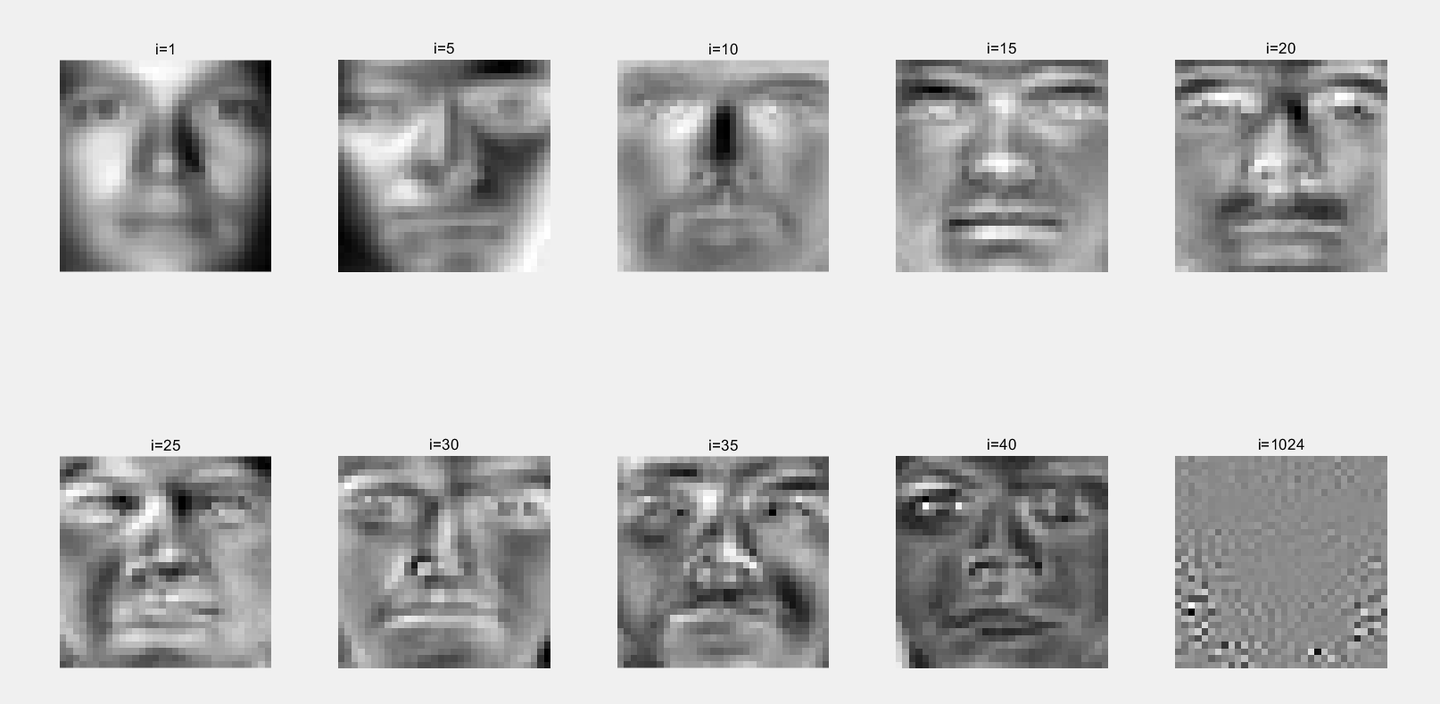
\includegraphics[width=0.8\textwidth]{Img/v2-62f392d4e1056457c15ccb4dd81dc539_1440w.png}
    \caption{Arranging eigenfaces according to eigenvalue size, it can be seen that eigenfaces with larger eigenvalues contain more effective information}
\end{figure}

\paragraph{Theoretical Basis of Eigenvalue Decomposition}
According to the spectral theorem in linear algebra, for a real symmetric matrix (the covariance matrix \( C \) is a real symmetric matrix), there exists an orthogonal matrix \( Q \) such that \( C = Q \Lambda Q^T \), where \( \Lambda \) is a diagonal matrix whose diagonal elements are the eigenvalues \( \lambda_i \) of \( C \), and the columns of \( Q \) are the corresponding eigenvectors \( v_i \). This theorem guarantees that we can diagonalize the covariance matrix \( C \) through eigenvalue decomposition, thereby finding the principal components of the data.

\paragraph{Selecting Principal Components}
Sort the eigenvalues in descending order, i.e., \( \lambda_1 \geq \lambda_2 \geq \cdots \geq \lambda_n \). According to the set principal component retention ratio (e.g., \texttt{KEEP\_COMPONENTS} is 0.95), select the first \( k \) eigenvectors as principal components, so that the cumulative contribution rate reaches the set ratio. The formula for calculating the cumulative contribution rate is:
\[
\sum_{i=1}^{k} \lambda_i / \sum_{i=1}^{n} \lambda_i \geq 0.95
\]
These \( k \) eigenvectors constitute the basis vectors of the eigenface space, which are used for subsequent data projection and feature extraction. Selecting the appropriate number of principal components is one of the key steps in PCA, as it requires a trade-off between retaining sufficient information and reducing data dimensionality. If too many principal components are retained, although more information can be retained, the dimensionality reduction effect is not obvious; if too few principal components are retained, important recognition features may be lost, leading to a decrease in recognition accuracy.

\paragraph{Data Projection}
Project the original face image vector \( x \) into the low-dimensional space formed by the selected eigenvectors to obtain the projected vector \( y \). The projection formula is:
\[
y = V^T (x - \mu)
\]
where \( V \) is the matrix composed of the first \( k \) eigenvectors, with each column being an eigenvector. Through projection, high-dimensional face image data is converted into low-dimensional feature vector representation, achieving dimensionality reduction. In the low-dimensional space, the computational and storage requirements of the data are greatly reduced, while the main variance information is still retained, allowing for effective face recognition.

\subsubsection{PCA Simple Data Example}

\begin{figure}[H]
    \centering
    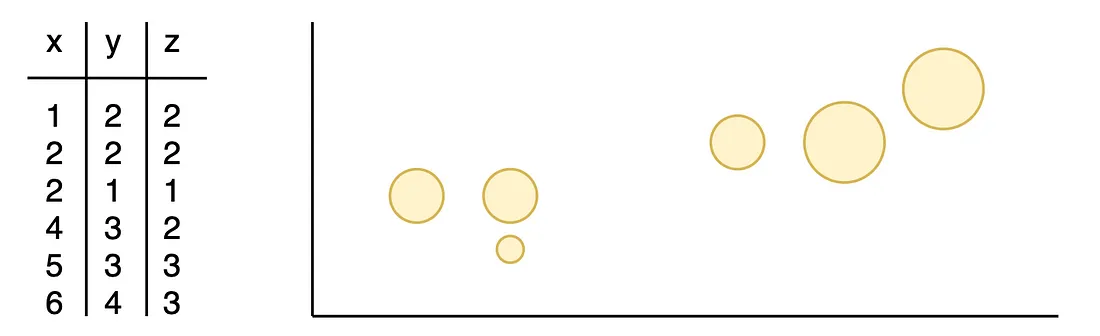
\includegraphics[width=0.7\textwidth]{Img/1_MJlSXELJ6-zNJibG5CtqIg.png}
    \caption{Plot data}
\end{figure}

\begin{figure}[H]
    \centering
    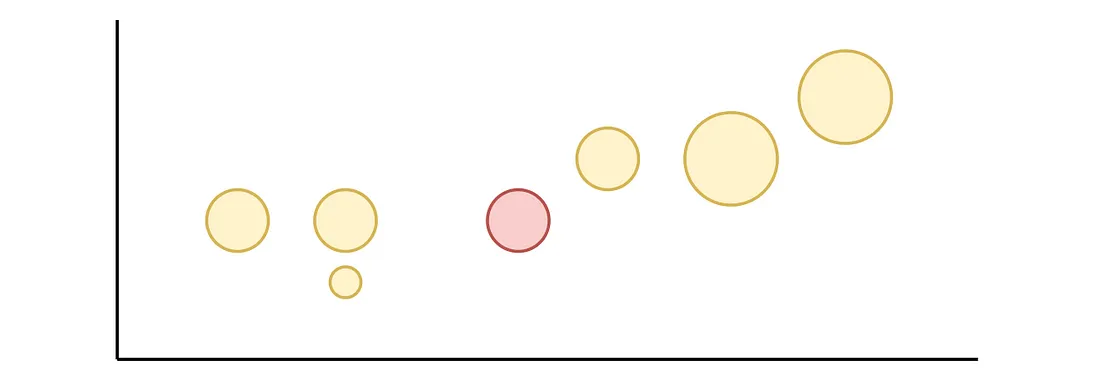
\includegraphics[width=0.7\textwidth]{Img/1_1BiMkGksH0JBOEOlf1tBTg.png}
    \caption{Find the centre of the data}
\end{figure}

\begin{figure}[H]
    \centering
    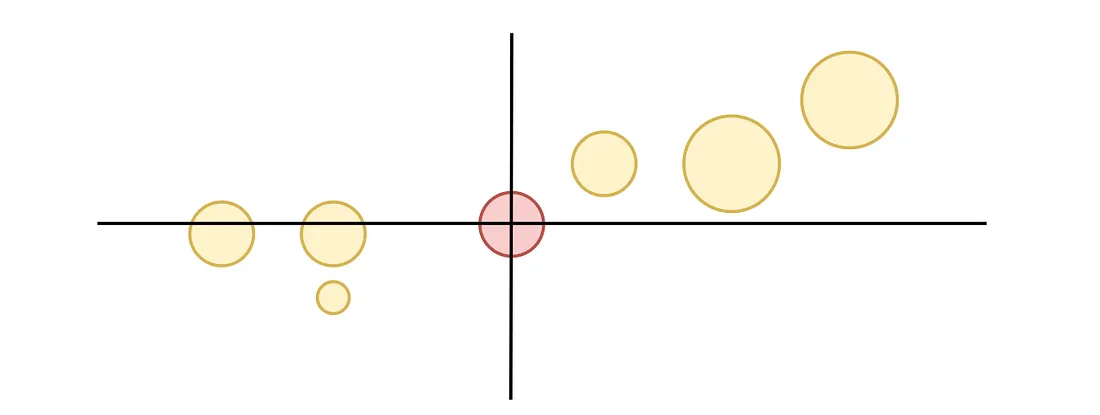
\includegraphics[width=0.7\textwidth]{Img/1_m3gnAUA9dBFQlbgWAziu3A.png}
    \caption{Shift the data points so the centre is now at (0, 0)}
\end{figure}

\begin{figure}[H]
    \centering
    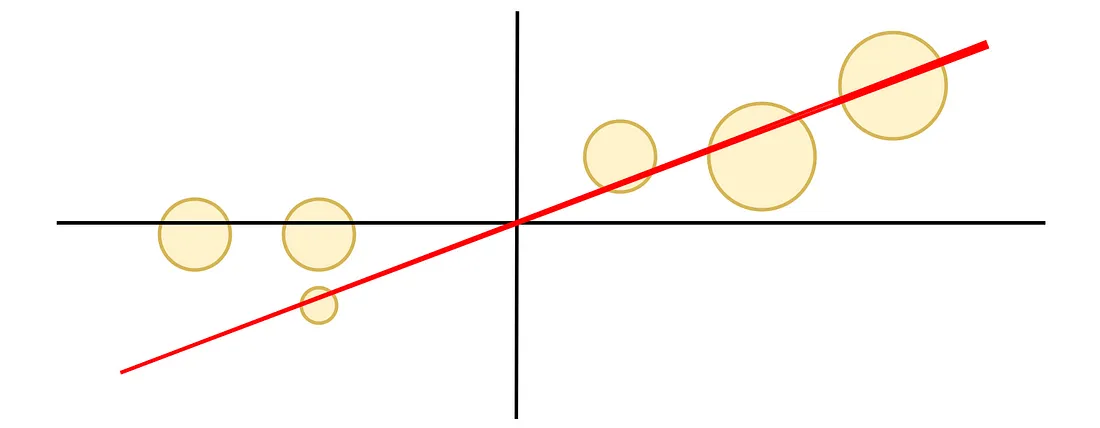
\includegraphics[width=0.7\textwidth]{Img/1_OjfIsQ5mxzfWoh3wtoBDBA.png}
    \caption{Find the line of best fit PC1}
\end{figure}

\begin{figure}[H]
    \centering
    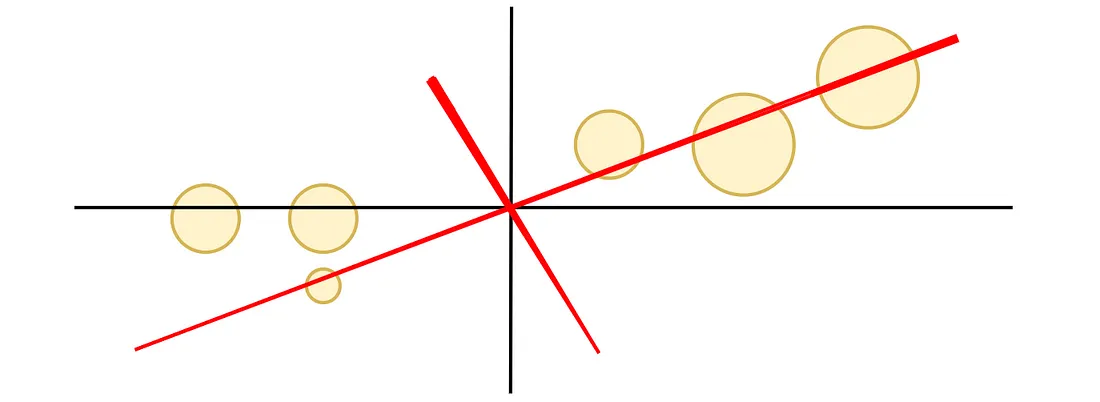
\includegraphics[width=0.7\textwidth]{Img/1_oRj5G874ukOev-uLrsq7LQ.png}
    \caption{Find another line PC2}
\end{figure}

\begin{figure}[H]
    \centering
    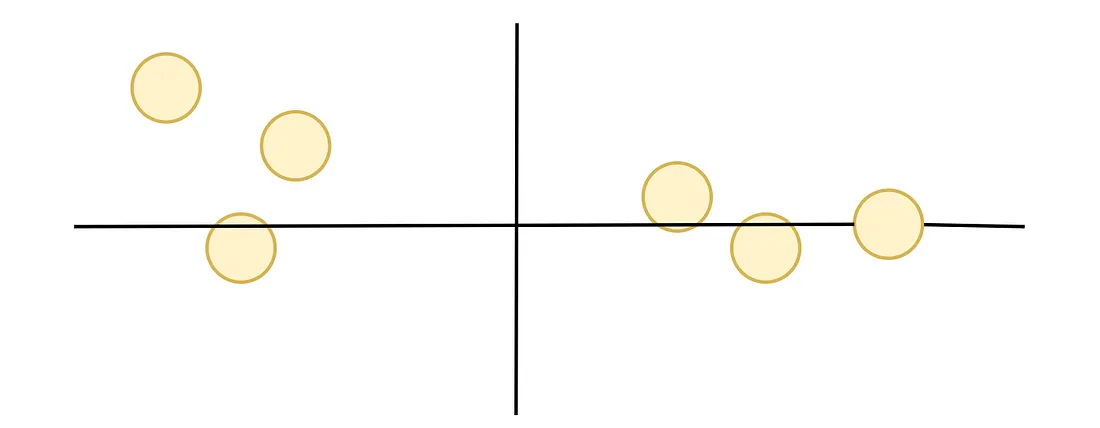
\includegraphics[width=0.7\textwidth]{Img/1_juLo2GtiuLdHhJOaNljyqw.png}
    \caption{Rotate the chart so PC1 is the x-axis and PC2 is the y-axis}
\end{figure}

\subsubsection{Efficient Methods for Calculating Eigenvectors in PCA}
In practical applications, directly calculating the eigenvectors of the covariance matrix of high-dimensional images is computationally infeasible. For example, for a \( 100 \times 100 \) grayscale image, each image is a point in a \( 10,000 \)-dimensional space, and the covariance matrix \( S \) has a size of \( 10,000 \times 10,000 \), with \( 10^8 \) elements. However, the rank of the covariance matrix is limited by the number of training images: if there are \( N \) training samples, there are at most \( N - 1 \) eigenvectors corresponding to non-zero eigenvalues. If the number of training samples is smaller than the dimensionality of the images, the calculation of eigenvectors can be simplified by the following method.

\paragraph{A. Data Matrix Construction and Preprocessing}
Let \( T \) be the matrix of preprocessed images, where each column corresponds to an image after subtracting the mean image. Assume we have \( N \) training samples, each sample is a \( D \)-dimensional vector (e.g., a \( 100 \times 100 \) image flattened into a \( 10,000 \)-dimensional vector), then the data matrix \( T \) has a size of \( D \times N \).

\paragraph{B. Calculating the Covariance Matrix}
The covariance matrix \( S \) can be expressed as:
\[
S = \frac{1}{N - 1} T T^T
\]
where \( T T^T \) is a \( D \times D \) matrix. Directly calculating the eigenvectors of this matrix is computationally infeasible, especially when \( D \) is large.

\paragraph{C. Simplifying Eigenvalue Decomposition}
To simplify the calculation, we can instead calculate the eigenvectors of \( T^T T \). Let the eigenvectors of \( T^T T \) be \( u_i \), with corresponding eigenvalues \( \lambda_i \), then:
\[
T^T T u_i = \lambda_i u_i
\]
If we multiply both sides of the equation by \( T \), we get:
\[
T T^T T u_i = \lambda_i T u_i
\]
This means that if \( u_i \) is an eigenvector of \( T^T T \), then \( v_i = T u_i \) is an eigenvector of \( S \). Since \( T^T T \) is an \( N \times N \) matrix, and usually \( N \) is much smaller than \( D \), calculating the eigenvectors of \( T^T T \) is much easier.

\paragraph{D. Normalizing Eigenvectors}
Note that the eigenvectors \( v_i \) obtained through the above method are not normalized. To ensure that the eigenvectors have unit length, we need to normalize \( v_i \):
\[
v_i = \frac{T u_i}{\|T u_i\|}
\]
where \( \|T u_i\| \) represents the norm of the vector \( T u_i \).

\paragraph{E. Computational Complexity Analysis}
Through the above method, we reduce the computational complexity from \( O(D^3) \) to \( O(N^3) \), where \( D \) is the dimensionality of the images and \( N \) is the number of training samples. Since \( N \) is usually much smaller than \( D \), this method greatly reduces the computational cost, making PCA feasible on high-dimensional data.

Assume we have 300 \( 100 \times 100 \) pixel images, each image flattened into a \( 10,000 \)-dimensional vector. Directly calculating the eigenvectors of a \( 10,000 \times 10,000 \) covariance matrix is computationally infeasible. Through the above method, we only need to calculate the eigenvectors of a \( 300 \times 300 \) matrix \( T^T T \), and then obtain the eigenvectors of the covariance matrix through simple matrix multiplication.

\subsubsection{Advantages of PCA in Face Recognition}
\begin{itemize}
    \item \textbf{Removing Redundant Information}: Face image data usually contains a large amount of redundant information, such as high correlation between adjacent pixels. PCA removes this redundant information by finding the principal components of the data, retaining only the most representative features, thereby improving recognition efficiency and accuracy.
    \item \textbf{Reducing the Curse of Dimensionality}: In high-dimensional spaces, data distribution is often sparse, leading to the "curse of dimensionality" problem, where the performance of classifiers decreases as dimensionality increases. PCA projects high-dimensional face image data into a low-dimensional space, effectively alleviating the curse of dimensionality and allowing classifiers to better learn and recognize the data.
    \item \textbf{Strong Feature Extraction Capability}: The eigenfaces extracted by PCA are the most variable directions in the data, capturing the main features of the face, such as facial contours, eyes, nose, mouth, etc. These features are important for face recognition and can improve recognition accuracy.
\end{itemize}

\subsection{K-Nearest Neighbors Reclassifier (kNNR)}

\subsubsection{Basic Principles of kNNR}
kNNR is an instance-based classification algorithm that plays a key role in the face recognition system. Its core idea is to find the \( k \) nearest neighbors of the sample to be recognized in the training set, and predict the category of the sample based on the category distribution of these \( k \) neighbors. In this system, by calculating the distance between the image to be recognized and all images in the training set, the \( k \) nearest samples are selected, and the category with the highest frequency among these \( k \) samples is used as the prediction result. If multiple categories have the same frequency, the category of the nearest sample is selected as the final prediction result.

\subsubsection{Mathematical Principles of kNNR}

\paragraph{Distance Metric}
Assume the training set contains \( N \) samples, each sample \( x_i \) has a corresponding category label \( y_i \). For the sample \( x \) to be recognized, calculate its distance \( d(x, x_i) \) to each sample \( x_i \) in the training set. The Euclidean distance is usually used as the metric, and the formula is:
\[
d(x, x_i) = \sqrt{\sum_{j=1}^{n} (x_j - x_{ij})^2}
\]
where \( x_j \) and \( x_{ij} \) are the \( j \)-th feature values of the sample \( x \) to be recognized and the training sample \( x_i \), respectively. The Euclidean distance is the most commonly used distance metric, as it intuitively reflects the geometric distance between two samples in the feature space. In face recognition, the Euclidean distance can measure the similarity between two face images in the feature space. The smaller the distance, the more similar the two images are.
\begin{figure}[H]
    \centering
    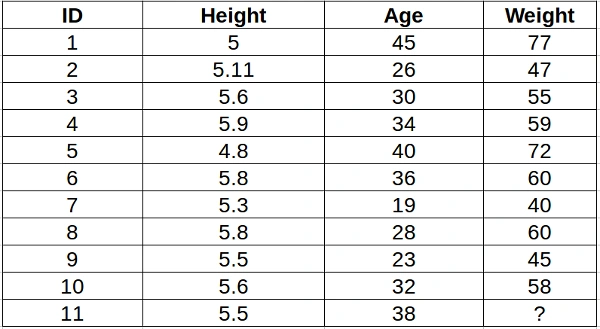
\includegraphics[width=0.7\textwidth]{Img/Screenshot-from-2018-08-22-15-03-42.png}
    \caption{Simple example table}
\end{figure}

\begin{figure}[H]
    \centering
    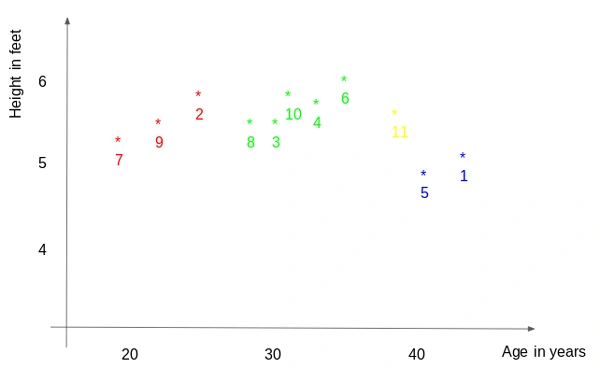
\includegraphics[width=0.7\textwidth]{Img/Screenshot-from-2018-08-22-12-49-19.png}
    \caption{Simple example coordinate graph}
\end{figure}


\begin{figure}[H]
    \centering
    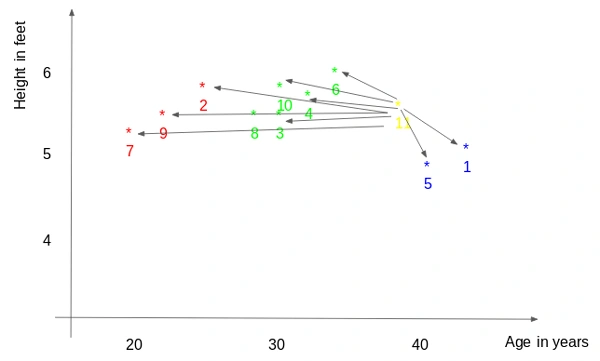
\includegraphics[width=0.7\textwidth]{Img/Screenshot-from-2018-08-22-12-49-33.png}
    \caption{Calculate the distance between the new point and each training point}
\end{figure}

\paragraph{Choosing the Value of \( k \)}
The choice of \( k \) is one of the key parameters of the kNNR algorithm. If \( k \) is too small, the model is easily affected by noise, leading to overfitting; if \( k \) is too large, the model becomes too smooth, ignoring local feature information, leading to underfitting. Usually, cross-validation can be used to select the appropriate \( k \) value, i.e., dividing different validation sets on the training set, testing different \( k \) values, and selecting the \( k \) value that achieves the highest classification accuracy on the validation set.

\begin{figure}[H]
    \centering
    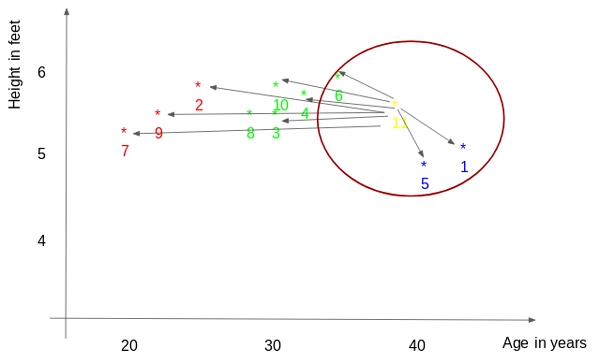
\includegraphics[width=0.7\textwidth]{Img/Screenshot-from-2018-08-22-12-50-04.png}
    \caption{For a value k = 3, the closest points are ID1, ID5, and ID6.}
\end{figure}

\begin{figure}[H]
    \centering
    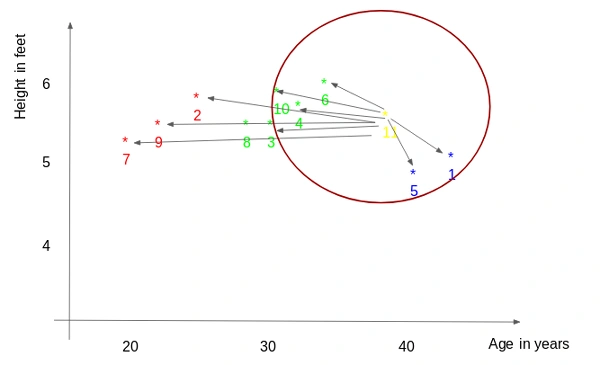
\includegraphics[width=0.7\textwidth]{Img/Screenshot-from-2018-08-22-12-50-16.png}
    \caption{For the value of k = 5, the closest point will be ID1, ID4, ID5, ID6, and ID10.}
\end{figure}

\paragraph{Voting Decision}
Select the \( k \) nearest neighbors of \( x \), and these \( k \) samples form a neighborhood. Count the frequency of each category in the neighborhood, and let the frequency of category \( c \) be \( n_c \). Predict the category of the sample \( x \) to be recognized as the category with the highest frequency, i.e.:
\[
\hat{y} = \arg\max_{c} n_c
\]
If multiple categories have the same frequency, i.e., there are multiple \( c \) such that \( n_c \) is the maximum, then among these categories, select the category of the sample closest to \( x \) as the predicted category of the sample \( x \).

\paragraph{Role of the Threshold}
In the face recognition system, the threshold is used to control the strictness of recognition. Specifically, the threshold determines the minimum distance between the sample to be recognized and the training samples. If the distance between the sample to be recognized and the nearest neighbor sample is less than the threshold, the recognition is considered successful; otherwise, the recognition fails, and the result "Stranger" is returned. The setting of the threshold directly affects the recognition accuracy and misrecognition rate of the system. A lower threshold increases the sensitivity of the system but may lead to more misrecognitions; a higher threshold improves the accuracy of the system but may lead to missed recognitions.

\paragraph{Dynamic Adjustment of the Threshold}
To adapt to different application scenarios and requirements, the system provides the function of dynamically adjusting the threshold. Users can adjust the threshold in real time through the slider control, observe the changes in recognition results, and find the most suitable threshold setting for the current scenario.

\subsubsection{Advantages of kNNR in Face Recognition}
\begin{itemize}
    \item \textbf{Simple and Easy to Understand}: The principle of the kNNR algorithm is simple and intuitive, and it does not require complex model training. It only needs to store training samples and corresponding category labels. During prediction, it only needs to calculate the distance between the sample to be recognized and the training samples, and then make a voting decision, making it easy to implement and understand.
    \item \textbf{Strong Adaptability}: The kNNR algorithm does not require assumptions about the distribution of the data and can adapt to various types of data. In face recognition, due to the diversity and complexity of face images, the data distribution is often complex, and the kNNR algorithm can handle this situation well, demonstrating strong adaptability.
    \item \textbf{Good Locality}: The kNNR algorithm is a classification algorithm based on local information. It only considers the neighboring samples of the sample to be recognized, capturing the local features of the data. In face recognition, local features are important for distinguishing different faces, and the kNNR algorithm can make full use of these local features to improve recognition accuracy.
\end{itemize}
\newpage
\section{Core Code and Explanation}

\subsection{PCA Core Code and Explanation}

\subsubsection{Code Snippet 1: PCA Data Preprocessing}
\begin{lstlisting}[basicstyle=\scriptsize\ttfamily, linewidth=\textwidth]
def fit(self, keep_components_ratio):
    # Calculate the mean face
    self.mean_face = self.train_matrix.mean(axis=1, keepdims=True)
    # Center the data
    self.centered_data = self.train_matrix - self.mean_face

    # Calculate the covariance matrix
    cov_matrix = np.dot(self.centered_data.T, self.centered_data) / (self.train_matrix.shape[1] - 1)
    # Eigenvalue decomposition
    eig_vals, eig_vecs = np.linalg.eig(cov_matrix)
    # Sort eigenvalues
    sorted_indices = np.argsort(eig_vals)[::-1]
    eig_vecs = eig_vecs[:, sorted_indices]
    eig_vals = eig_vals[sorted_indices]

    # Calculate the cumulative variance contribution rate
    eig_vals_total = np.sum(eig_vals)
    variance_explained = np.cumsum(eig_vals) / eig_vals_total
    # Select the number of principal components
    num_components = np.argmax(variance_explained >= keep_components_ratio) + 1

    # Select the first k eigenvectors
    eig_vecs = eig_vecs[:, :num_components]
    # Calculate eigenfaces
    self.eigenfaces = np.dot(self.centered_data, eig_vecs)
    # Normalize eigenfaces
    eigenface_norms = np.linalg.norm(self.eigenfaces, axis=0, keepdims=True)
    eigenface_norms[eigenface_norms == 0] = 1
    self.eigenfaces /= eigenface_norms
\end{lstlisting}

\subsubsection{Explanation of Code Snippet 1}
\begin{itemize}
    \item \textbf{Mean Face Calculation}:
    \begin{itemize}
        \item The mean face is the average feature of all face images, reflecting the basic structure of the face. By calculating the mean face, we can align all face images to a common center point, facilitating subsequent feature extraction.
        \item In the code, \texttt{self.mean\_face = self.train\_matrix.mean(axis=1, keepdims=True)} calculates the mean face of the training data.
        \item \texttt{self.centered\_data = self.train\_matrix - self.mean\_face} centers the data, making the data distribution centered at the origin.
    \end{itemize}
    \item \textbf{Covariance Matrix Calculation}:
    \begin{itemize}
        \item The covariance matrix reflects the correlation between different dimensions of the data. In face recognition, the covariance matrix describes the correlation between different pixels of the face image.
        \item In the code, \texttt{cov\_matrix = np.dot(self.centered\_data.T, self.centered\_data) / (self.train\_matrix.shape[1] - 1)} calculates the covariance matrix of the centered data.
    \end{itemize}
    \item \textbf{Eigenvalue Decomposition}:
    \begin{itemize}
        \item Eigenvalue decomposition is the core step of PCA. By decomposing the covariance matrix, we can obtain eigenvalues and eigenvectors. Eigenvalues represent the variance of the data in different directions, and eigenvectors represent the direction of data variation.
        \item In the code, \texttt{eig\_vals, eig\_vecs = np.linalg.eig(cov\_matrix)} performs eigenvalue decomposition on the covariance matrix.
        \item \texttt{sorted\_indices = np.argsort(eig\_vals)[::-1]} sorts the eigenvalues in descending order.
    \end{itemize}
    \item \textbf{Selecting Principal Components}:
    \begin{itemize}
        \item Principal components are the most variable directions in the data. Selecting the appropriate number of principal components can retain sufficient information while reducing data dimensionality.
        \item In the code, \texttt{variance\_explained = np.cumsum(eig\_vals) / eig\_vals\_total} calculates the cumulative variance contribution rate.
        \item \texttt{num\_components = np.argmax(variance\_explained >= keep\_components\_ratio) + 1} selects the number of principal components based on the set retention ratio (e.g., 95\%).
    \end{itemize}
    \item \textbf{Eigenface Calculation}:
    \begin{itemize}
        \item Eigenfaces are the key features extracted by PCA, representing the most variable directions in the face image.
        \item In the code, \texttt{self.eigenfaces = np.dot(self.centered\_data, eig\_vecs)} projects the centered data into the eigenvector space to obtain eigenfaces.
    \end{itemize}
\end{itemize}

\subsection{kNN Core Code and Explanation}

\subsubsection{Code Snippet 2: kNN Classifier}
\begin{lstlisting}[basicstyle=\scriptsize\ttfamily, linewidth=\textwidth]
def kNNR_classifier(self, distances, k, train_labels):
    # Find the k nearest neighbors
    knn_indices = np.argpartition(distances, k - 1)[:k]
    knn_labels = train_labels[knn_indices]

    # Count the frequency of each label in the k neighbors
    unique_labels, counts = np.unique(knn_labels, return_counts=True)
    max_count = counts.max()
    candidate_labels = unique_labels[counts == max_count]

    # Handle ties
    best_index = None
    best_distance = float('inf')
    for label in candidate_labels:
        indices = knn_indices[knn_labels == label]
        local_idx = indices[np.argmin(distances[indices])]
        if distances[local_idx] < best_distance:
            best_distance = distances[local_idx]
            best_index = local_idx

    return best_index
\end{lstlisting}

\subsubsection{Explanation of Code Snippet 2}
\begin{itemize}
    \item \textbf{Selecting Nearest Neighbors}:
    \begin{itemize}
        \item The core idea of the kNN algorithm is to calculate the distance between the sample to be recognized and the training samples, and find the k nearest neighbors.
        \item In the code, \texttt{knn\_indices = np.argpartition(distances, k - 1)[:k]} finds the indices of the k nearest neighbors.
        \item \texttt{knn\_labels = train\_labels[knn\_indices]} retrieves the labels of these k neighbors.
    \end{itemize}
    \item \textbf{Voting Decision}:
    \begin{itemize}
        \item Among the k neighbors, count the frequency of each label, and select the label with the highest frequency as the prediction result.
        \item In the code, \texttt{unique\_labels, counts = np.unique(knn\_labels, return\_counts=True)} counts the frequency of each label in the k neighbors.
        \item \texttt{max\_count = counts.max()} finds the label with the highest frequency.
    \end{itemize}
    \item \textbf{Handling Ties}:
    \begin{itemize}
        \item If multiple labels have the same frequency, select the label of the sample closest to the sample to be recognized as the final prediction result.
        \item In the code, \texttt{best\_index = None} and \texttt{best\_distance = float('inf')} are used to record the index of the closest sample.
    \end{itemize}
\end{itemize}

\subsection{Face Detection Core Code and Explanation}

\subsubsection{Code Snippet 3: Face Detection}
\begin{lstlisting}[basicstyle=\scriptsize\ttfamily, linewidth=\textwidth]
def detect_faces(self, image):
    (h, w) = image.shape[:2]
    blob = cv2.dnn.blobFromImage(cv2.resize(image, (300, 300)), 1.0, (300, 300), (104.0, 177.0, 123.0))
    self.net.setInput(blob)
    return self.net.forward()
\end{lstlisting}

\subsubsection{Explanation of Code Snippet 3}
\begin{itemize}
    \item \textbf{Image Preprocessing}:
    \begin{itemize}
        \item The first step in face detection is to resize the input image to a fixed size (e.g., 300x300) and normalize it.
        \item In the code, \texttt{blob = cv2.dnn.blobFromImage(...)} resizes the input image to 300x300 and normalizes it.
    \end{itemize}
    \item \textbf{Face Detection}:
    \begin{itemize}
        \item Use a pre-trained deep learning model to perform face detection and return the detection results.
        \item In the code, \texttt{self.net.setInput(blob)} inputs the preprocessed image into the neural network.
        \item \texttt{return self.net.forward()} returns the face detection results from the neural network.
    \end{itemize}
\end{itemize}

\subsection{Dataset Processing Core Code and Explanation}

\subsubsection{Code Snippet 4: Dataset Splitting}
\begin{lstlisting}[basicstyle=\scriptsize\ttfamily, linewidth=\textwidth]
def split_dataset(self, matrix, labels, train_ratio):
    train_data = []
    train_labels = []
    test_data = []
    test_labels = []
    for label in np.unique(labels):
        indices = np.where(labels == label)[0]
        indices = np.random.permutation(indices)
        train_num = int(len(indices) * train_ratio)
        train_indices = indices[:train_num]
        test_indices = indices[train_num:]
        train_data.append(matrix[:, train_indices])
        test_data.append(matrix[:, test_indices])
        train_labels.extend([label] * len(train_indices))
        test_labels.extend([label] * len(test_indices))

    train_data = np.hstack(train_data)
    test_data = np.hstack(test_data)
    train_labels = np.array(train_labels)
    test_labels = np.array(test_labels)
    return train_data, train_labels, test_data, test_labels
\end{lstlisting}

\subsubsection{Explanation of Code Snippet 4}
\begin{itemize}
    \item \textbf{Dataset Splitting}:
    \begin{itemize}
        \item Split the dataset into training and testing sets according to the set training ratio (e.g., 80\%).
        \item In the code, \texttt{train\_num = int(len(indices) * train\_ratio)} calculates the number of training samples for each category.
        \item \texttt{train\_indices = indices[:train\_num]} and \texttt{test\_indices = indices[train\_num:]} obtain the indices of the training and testing sets, respectively.
    \end{itemize}
    \item \textbf{Data Merging}:
    \begin{itemize}
        \item Merge the training and testing data of each category into complete training and testing sets.
        \item In the code, \texttt{train\_data = np.hstack(train\_data)} and \texttt{test\_data = np.hstack(test\_data)} merge the data of each category.
    \end{itemize}
\end{itemize}

\subsection{Image Preprocessing Core Code and Explanation}

\subsubsection{Code Snippet 5: Image Enhancement}
\begin{lstlisting}[basicstyle=\scriptsize\ttfamily, linewidth=\textwidth]
def enhance_image(self, image, remove_background=True):
    ycrcb_face = cv2.cvtColor(image, cv2.COLOR_BGR2YCR_CB)
    channels = cv2.split(ycrcb_face)
    channels = list(channels)
    clahe = cv2.createCLAHE(clipLimit=2.0, tileGridSize=(8, 8))
    channels[0] = clahe.apply(channels[0])
    cv2.merge(channels, ycrcb_face)
    image = cv2.cvtColor(ycrcb_face, cv2.COLOR_YCR_CB2BGR)
    if remove_background:
        blurred_face = cv2.GaussianBlur(image, (7, 7), 0)
        mask = np.zeros(image.shape[:2], np.uint8)
        bgd_model = np.zeros((1, 65), np.float64)
        fgd_model = np.zeros((1, 65), np.float64)
        rect = (int(Config.RECOGNITION_SIZE * 0.04),
                int(Config.RECOGNITION_SIZE * 0.04),
                image.shape[1] - int(Config.RECOGNITION_SIZE * 0.08),
                image.shape[0] - int(Config.RECOGNITION_SIZE * 0.08))
        cv2.grabCut(blurred_face, mask, rect, bgd_model, fgd_model, 1, cv2.GC_INIT_WITH_RECT)
        mask2 = np.where((mask == cv2.GC_FGD) | (mask == cv2.GC_PR_FGD), 1, 0).astype('uint8')
        grabbed_face = image * mask2[:, :, np.newaxis]
        image = cv2.cvtColor(grabbed_face, cv2.COLOR_BGR2GRAY)
    else:
        image = cv2.cvtColor(image, cv2.COLOR_BGR2GRAY)
    return image
\end{lstlisting}

\subsubsection{Explanation of Code Snippet 5}
\begin{itemize}
    \item \textbf{Image Enhancement}:
    \begin{itemize}
        \item Use CLAHE (Contrast Limited Adaptive Histogram Equalization) to enhance the contrast of the image, making facial features more prominent.
        \item In the code, \texttt{clahe = cv2.createCLAHE(clipLimit=2.0, tileGridSize=(8,8))} creates a CLAHE object.
        \item \texttt{channels[0] = clahe.apply(channels[0])} enhances the brightness channel of the image.
    \end{itemize}
    \item \textbf{Background Removal}:
    \begin{itemize}
        \item Use the GrabCut algorithm to remove the image background, retaining the face region and reducing the interference of the background on recognition results.
        \item In the code, \texttt{cv2.grabCut(...)} uses the GrabCut algorithm to remove the background.
        \item \texttt{mask2 = np.where((mask == cv2.GC\_FGD) | (mask == cv2.GC\_PR\_FGD), 1, 0).astype('uint8')} generates the background mask.
        \item \texttt{grabbed\_face = image * mask2[:, :, np.newaxis]} retains the foreground region.
    \end{itemize}
\end{itemize}
\newpage
\section{Project Recognition Results Analysis}

\subsection{Local Dataset Testing}

\begin{table}[H]
    \centering
    \begin{tabular}{|c|c|c|c|c|}
        \hline
        Dataset & Test Samples & Correct Recognitions & Recognition Rate & Notes \\
        \hline
        Att\_Faces & Train 120, Test 30 & 23 & 76.66\% & No background interference, higher recognition rate. \\
        \hline
        Dataset\_Pure & Train 100, Test 25 & 18 & 72\% & No background interference, higher recognition rate. \\
        \hline
    \end{tabular}
    \caption{Local Dataset Testing Results}
\end{table}

\subsection{Camera Testing}

\begin{table}[H]
    \centering
    \begin{tabular}{|c|c|c|}
        \hline
        & With Background & Remove Background \\
        \hline
        Conditions & Strict background requirements & No strict background requirements \\
        \hline
        Recognition Rate & Stable recognition at specific angles & Faster and more accurate recognition \\
        \hline
        Screenshot & 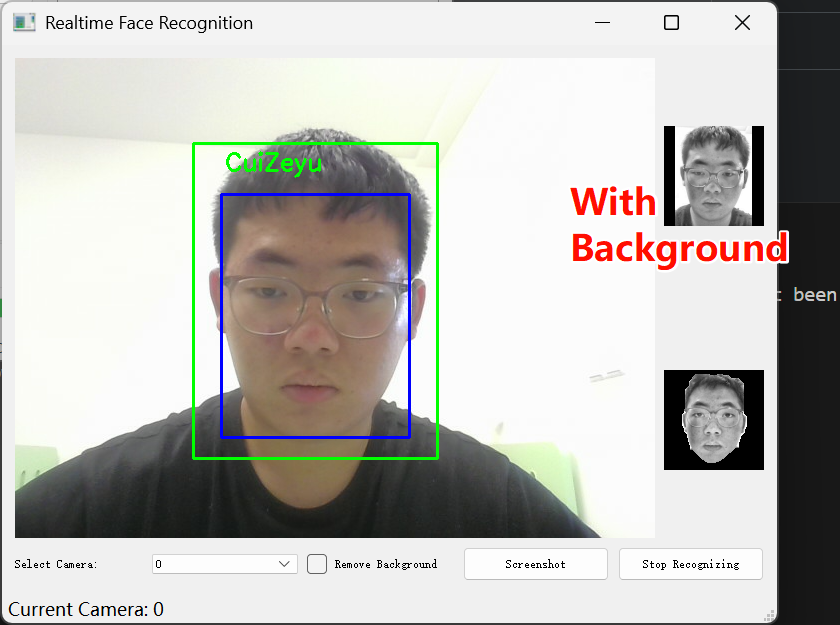
\includegraphics[width=0.4\textwidth]{Img/PixPin_2025-03-09_11-53-03.png} & 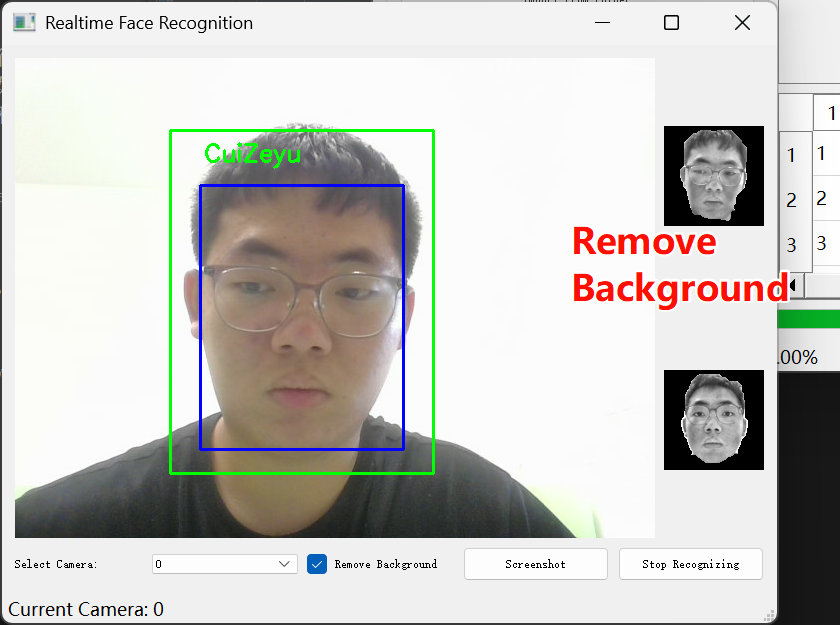
\includegraphics[width=0.4\textwidth]{Img/PixPin_2025-03-09_11-54-41.png} \\
        \hline
    \end{tabular}
    \caption{Camera Testing Results}
\end{table}
\newpage
\section{Application Scenarios}

\subsection{Security Surveillance}

\subsubsection{Public Safety}
In transportation hubs such as airports, train stations, and subway stations, where there is frequent and complex human traffic, this PCA-based face recognition system can be used for real-time identity monitoring. The system can be connected to surveillance cameras to quickly identify individuals entering the premises. Once a blacklisted individual is detected, the system can immediately issue an alert, notifying security personnel to take appropriate measures.

\subsubsection{Residential and Corporate Security}
For residential communities and corporate office areas, the system can be an important component of the access control system. Residents or employees can simply pass through the face recognition device for identity verification when entering the community or office area, and the system can quickly determine whether they are authorized personnel.

\subsubsection{Dynamic Threshold Adjustment for Different Scenarios}
In security surveillance scenarios, different environmental conditions (such as lighting, camera angles, etc.) may affect the accuracy of face recognition. The system's threshold adjustment function allows security personnel to dynamically adjust the recognition threshold according to actual conditions. For example, in low-light environments, the threshold can be appropriately lowered to improve recognition sensitivity; in well-lit environments, the threshold can be appropriately raised to reduce misidentifications.

\subsection{Financial Payment}

\subsubsection{Face Payment}
In mobile payment scenarios, the system can be used for identity verification in face payment. When a user performs a payment operation, they only need to face the camera of the payment device, and the system will compare the user's facial features with the pre-registered facial information.

\subsubsection{Bank Account Opening and Identity Verification}
Banks can use this face recognition system to verify customer identity when opening accounts. By capturing the customer's face image and comparing it with the photo on the ID card, the system ensures the authenticity of the account holder's identity. Additionally, in subsequent business operations such as large withdrawals or transfers, face recognition can be used for identity verification, further ensuring the security of customer funds.

\subsection{Education}

\subsubsection{Attendance Management}
Schools can use this system for student attendance management. Face recognition devices installed at classroom entrances can automatically recognize students' identities and record attendance information when they enter the classroom. This avoids issues such as proxy attendance and missed attendance in traditional attendance methods, improving the accuracy and efficiency of attendance management. Teachers can view students' attendance status through the system at any time, keeping track of students' attendance in real time.

\subsubsection{Exam Proctoring}
During exams, the face recognition system can be used to verify the identity of candidates, preventing impersonation. Before entering the exam room, candidates must pass through the face recognition device for identity confirmation, and the system will compare the captured face image with the photo from the candidate's registration.
\newpage
\section{Project Summary}

\subsection{Project Results Summary and Analysis}
This project successfully designed and implemented a PCA-based face recognition system. By comprehensively applying PCA for feature extraction and the kNNR algorithm for classification and recognition, the system effectively completed the task of face image recognition. The system demonstrated high performance and accuracy in data processing, feature extraction, and classification recognition, while also providing a good user experience and scalability.

In the data processing stage, the system adopted flexible preprocessing strategies, including image cropping, resizing, and background removal, improving the quality of the image data. The automatic selection mechanism for PCA parameters ensured that key features were retained while effectively reducing data dimensionality, achieving a balance between computational efficiency and recognition accuracy. The simplicity and strong adaptability of the kNNR algorithm allowed the system to handle different types of face data well.

The threshold adjustment function provided by the project greatly enhanced the system's flexibility and applicability. Users can dynamically adjust the recognition threshold according to different application scenarios and requirements to achieve the best recognition results. This function not only improved the system's practicality but also provided users with more operational freedom, allowing the system to better adapt to complex and changing real-world environments.

Through the user interface developed based on \texttt{PyQt5}, the system achieved a high level of integration. Users can easily perform operations such as data import, model training, camera operations, and dataset management. The system also provides dataset saving and loading functions, making it convenient for users to manage and reuse data.

\subsection{Limitations Analysis}
Although the system has achieved certain results, there are still some limitations. In complex environments, such as severe lighting changes, large face poses, or occlusions, the system's recognition accuracy may be affected. This is because PCA mainly relies on global features and has relatively weak ability to capture local features. Additionally, the kNNR algorithm has high computational complexity when processing large datasets, leading to slower recognition speeds.

\subsection{Future Prospects}
To further improve the system's performance and applicability, future work can focus on the following aspects:

\begin{itemize}
    \item \textbf{Introducing Deep Learning Techniques}: Further research and experimentation with more complex and advanced deep learning models, such as Convolutional Neural Networks (CNN) and face recognition-specific networks (e.g., FaceNet, ArcFace), for feature extraction and classification. Deep learning models can automatically learn richer and more discriminative features, providing better recognition performance in complex environments.
    \item \textbf{Multimodal Fusion}: Combining face recognition with other biometric technologies (e.g., fingerprint recognition, iris recognition) to improve the system's security and reliability. Multimodal recognition can leverage the advantages of different biometric features, reducing the limitations of single-feature recognition.
    \item \textbf{Optimizing Algorithm Performance}: Addressing the high computational complexity of the kNNR algorithm by researching and adopting more efficient algorithms or data structures, such as KD-trees or ball trees, to accelerate the nearest neighbor search process and improve recognition speed.
    \item \textbf{Expanding Application Scenarios}: Further exploring the system's applications in more fields, such as smart homes, intelligent security, and healthcare. Customizing the system according to the needs of different application scenarios to improve its versatility and practicality.
\end{itemize}

Overall, this PCA-based face recognition system provides a solid foundation for subsequent research and development. Through continuous optimization and expansion, it is expected to play a greater role in the field of face recognition.

\section*{References}
\begin{itemize}
    \item \href{https://en.wikipedia.org/wiki/K-nearest_neighbors_algorithm}{k-nearest neighbors algorithm}
    \item \href{https://en.wikipedia.org/wiki/Principal_component_analysis}{Principal component analysis}
    \item \href{https://zh.wikipedia.org/wiki/%E7%89%B9%E5%BE%81%E8%84%B8}{特征脸}
    \item \href{https://zhuanlan.zhihu.com/p/356640804}{基于 PCA 的人脸识别方法——特征脸法}
    \item \href{https://medium.com/towards-data-science/pca-principal-component-analysis-explained-visually-in-5-minutes-20ce8a9ebf0f}{PCA (Principal Component Analysis) Explained Visually In 5 Minutes}
    \item \href{https://www.analyticsvidhya.com/blog/2018/08/k-nearest-neighbor-introduction-regression-python}{KNN algorithm: Introduction to K-Nearest Neighbors Algorithm for Regression}
\end{itemize}

\end{document}